%%%% ijcai19-multiauthor.tex

\typeout{IJCAI-19 Multiple authors example}

% These are the instructions for authors for IJCAI-19.

\documentclass{article}
\pdfpagewidth=8.5in
\pdfpageheight=11in
% The file ijcai19.sty is NOT the same than previous years'
\usepackage{ijcai19}

% Use the postscript times font!
\usepackage{times}
\renewcommand*\ttdefault{txtt}
\usepackage{soul}
\usepackage{url}
\usepackage[hidelinks]{hyperref}
\usepackage[utf8]{inputenc}
\usepackage[small]{caption}
\usepackage{graphicx}
\usepackage{amsmath}
\usepackage{booktabs}
\urlstyle{same}
%%%%%%%%%%%%%%%%%%%%%%%%%%%%%%%%%%%%%%%%%%%%%%%%%%%%%%%%%%%%%%%%%%%%%%%%
% OUR PACKAGES
%%%%%%%%%%%%%%%%%%%%%%%%%%%%%%%%%%%%%%%%%%%%%%%%%%%%%%%%%%%%%%%%%%%%%%%%

\usepackage{times}
% Optional math commands from https://github.com/goodfeli/dlbook_notation.
\input{math_commands.tex}
\usepackage{hyperref}
\usepackage{xspace}
\usepackage{url}
\usepackage{subfigure}
\usepackage{verbatim}
\usepackage{listings}
\usepackage{todonotes}
\usepackage{tikz}
\newcommand{\veronika}[1]{\todo[inline,author=Veronika,color=lightgray]{#1}}
\newcommand{\cristina}[1]{\todo[inline,author=Cristina,color=cyan]{#1}}

\newcommand{\support}{\text{support}\xspace}
\newcommand{\tool}{\text{RuDa}\xspace}
\newcommand{\nowa}{\ensuremath{n_{\text{OW}}}\xspace}
\newcommand{\nnoise}{\ensuremath{n_{\text{Noise}}}\xspace}
\newcommand{\ndag}{\ensuremath{n_{\text{DG}}}\xspace}
\newcommand{\nnskip}{\ensuremath{n_{\text{Skip}}}\xspace}
\newcommand{\db}{\ensuremath{\mathbb{D}}\xspace}%_{\text{CW}}
\newcommand{\dbowa}{\ensuremath{\db_{\text{OW}}}\xspace}
\newcommand{\dbowan}{\ensuremath{\db_{\text{OW+Noise}}}\xspace}
\newcommand{\dbn}{\ensuremath{\db_{\text{Noise}}}\xspace}
\newcommand{\sfacts}{\ensuremath{\mathbb{S}}\xspace}
\newcommand{\cfacts}{\ensuremath{\mathbb{C}}\xspace}
\newcommand{\tfacts}{\ensuremath{\mathbb{T}}\xspace}
%\newcommand{\fi}[1]{\textit{#1}}
\newcommand{\ass}{\text{ :- }}
\newcommand{\expred}[1]{\textrm{#1}\xspace}
\newcommand{\exconst}[1]{\textrm{#1}\xspace}
%%%%%%%%%%%%%%%%%%%%%%%%%%%%%%%%%%%%%%%%%%%%%%%%%%%%%%%%%%%%%%%%%%%%%%%%
%%%%%%%%%%%%%%%%%%%%%%%%%%%%%%%%%%%%%%%%%%%%%%%%%%%%%%%%%%%%%%%%%%%%%%%%
%%%%%%%%%%%%%%%%%%%%%%%%%%%%%%%%%%%%%%%%%%%%%%%%%%%%%%%%%%%%%%%%%%%%%%%%
%TODO DELETE IN FINAL VERSION
%https://www.overleaf.com/learn/latex/Questions/What_does_%22%5Cpdfendlink_ended_up_in_different_nesting_level_than_%5Cpdfstartlink%22_mean%3F
\hypersetup{draft}


\title{RuLeS: Synthetic Datasets for Rule Learning}% and evaluation tool?}
%\tool: Rule Learning Dataset Generation and Evaluation}

\author{
Submission \# 2728
%First Author$^1$\footnote{Contact Author}\and
%Second Author$^2$\and
%Third Author$^{2,3}$\And
%Fourth Author$^4$\\
%\affiliations
%$^1$First Affiliation\\
%$^2$Second Affiliation\\
%$^3$Third Affiliation\\
%$^4$Fourth Affiliation\\
%\emails
%\{first, second\}@example.com,
%third@other.example.com,
%fourth@example.com
}



\begin{document}


\maketitle


%%%%%%%%%%%%%%%%%%%%%%%%%%%%%%%%%%%%%%%%%%%%%%%%%
%IJCAI: six pages for the main text of the paper% 
%%%%%%%%%%%%%%%%%%%%%%%%%%%%%%%%%%%%%%%%%%%%%%%%%

\begin{abstract}
Logical rules are a popular knowledge representation language in many domains, they represent background knowledge and encode information that can be derived from given facts in a compact form.
%and allow for logical reasoning
% However, 
But rule formulation is complex and requires domain expertise,
and today's %often 
%large, heterogeneous, and incomplete 
knowledge graphs represent additional challenges.
Several approaches for automation, 
learning rules based on example facts,
% %solving 
% %the tedious task % in an automated fashion 
% inducing logic programs %VERONIKA should be known at IJCAI logical rules (also, logic programs) 
% from example facts (ILP), 
have been proposed over time,
including neural systems recently.
%Neural systems solve the tedious task by inducing logical rules (also, logic programs) from example facts. 
Yet, the area is missing adequate evaluation approaches: existing datasets (i.e., facts and the rules to be learned) resemble toy examples that neither cover the various kinds of dependencies between rules nor allow for testing scalability.
We present a %the \tool 
tool for generating %different kinds of 
datasets and for evaluating rule learning systems.
%ing neural inductive logic programming.
\end{abstract}
\section{Introduction}


Logical rules are a popular knowledge representation language in many domains. They represent %background 
domain knowledge, encode information that can be derived from given facts in a compact form, and allow for logical reasoning.
For example, given facts $\expred{parent}(\exconst{ann},\exconst{bob})$ and $\expred{parent}(\exconst{bob},\exconst{dan})$, the \emph{Datalog rule} 
$\expred{grandparent}(X,Z)\ass\expred{parent}(X,Y),\expred{parent}(Y,Z)$, encodes the fact $\expred{grandparent}(\exconst{ann},\exconst{dan})$ and describes its dependency on the other facts. Moreover, if the data grows and new facts are added, we can automatically derive new knowledge.
% 
Since rule formulation is complex and requires domain expertise,
\emph{rule learning} \cite{Raedt-08-Logical-and-relational-learning,Fuernkranz+-12-Foundations-of-Rule-Learning} %,SteGaHo-RR18:overview} 
has been an active research in AI for a long time %However, the classical approaches do not scale struggled with the  and has r
and recently revived with the application of deep learning. % approaches.

In the area of %\emph
{inductive logic programming}~(ILP) \cite{Muggleton-NGC91:ilp}, %this tedious task is solved by inducing 
the goal is to induce logical rules (also, logic programs) based on example facts. 
Classical ILP systems such as FOIL \cite{Quinlan-ML90:foil} and Progol \cite{Muggleton-NGC95:progol} usually apply exhaustive algorithms to mine rules for the given data and either require negative facts as
counter-examples or assume a closed world (for an overview of classical ILP systems see Table~2 in \cite{SteGaHo-RR18:overview}).
The \emph{closed-world assumption} (CWA) basically states that all facts % given are considered as true and 
that are not explicitly given as true are assumed to be false.
%, if given facts match a rule's conditions, then the consequences of the rule have to be also true in the real world.

Today, however, knowledge graphs (KGs) with their often incomplete, noisy, heterogeneous, and, especially, large amounts of data raise %completely 
new problems and require new solutions.
For instance, real data most often only partially satisfies the CWA %this assumption 
and does not contain counter-examples. Moreover, in an open world, absent facts cannot be considered as counter-examples either since they are not considered as false.
Therefore, the successor systems, with AMIE+ \cite{Galarraga+-VLDBJ15:amiep} and RDF2Rules \cite{WangLi-CoRR15:rdf2rules} as the most prominent representatives, 
assume the data to be only partially complete and
focus on rule learning in the sense of mining patterns that occur frequently in the data.
% This is the central challenge of our
% setting: to provide counterexamples for the rule mining.
% Since they lack scalability,
Furthermore, they implement advanced optimization approaches that make them applicable in wider scenarios. %eg use pruning, in-memory indexing
% 
In this way, they address already many of the issues that arise with today's knowledge graphs. Yet, their processing is still exhaustive.

% Today, however, knowledge graphs with their often incomplete, noisy, heterogeneous, and, especially, large amounts of data raise %completely 
% new problems and require new solutions.

%Ho+-ISWC18:guided-by-embedding,
%\emph{rule learning} \cite{Raedt-08-Logical-and-relational-learning,Fuernkranz+-12-Foundations-of-Rule-Learning},
Recently, {neural rule learning} approaches have been proposed  \cite{YaYaCo-NIPS17:neurallp,RoR-NIPS17,EGre-jair18:learning-explanatory-rules,Minervini+-NAMPI18:ntp-at-scale,OWaWa-IJCAI18:scalable-rule-learning,Campero+-corr18,Dong+-ICLR19:nlms} and they might be a good alternative %for learning rules % representations} 
since deep learning has coped with vast amounts of noisy and heterogeneous data already.
% have shown to provide solutions since 
The proposed solutions consider vector or matrix embeddings of symbols, facts and/or rules, and model inference using differentiable operations such as vector addition and matrix composition. However, the proposed methods are still premature: they only learn certain kinds of rules or lack scalability (e.g., because they search the entire rule space) and hence cannot compete with established rule mining systems such as AMIE+ yet, as shown in \cite{OWaWa-IJCAI18:scalable-rule-learning}, for example. 
%, or simply produce unsatisfactory results.
Further, the reported results are questionable in terms of generalization:
% , especially w.r.t.\ practice: %transferability to practice: 
the test datasets (i.e., facts and the rules to be learned) either resemble toy examples that neither cover the various kinds of possible dependencies in rule sets nor allow for testing scalability, or they do not contain any rules at all because there simply are no rules yet for the popular, publicly available KGs (see, e.g., the evaluations in \cite{EGre-jair18:learning-explanatory-rules} and \cite{OWaWa-IJCAI18:scalable-rule-learning}).
%daria: To the best of our knowledge, existing methods are purely statistics-based, i.e., they reduce the rule learning problem to algebraic operations on neural-embedding-based representations of a given KG
\veronika{not 1000\% sure (doesn't seem so), can Dong et al %\cite{Dong+-ICLR19:nlms} 
output the rules? if not, delete reference above}

We are hence in a chicken-and-egg situation missing rules for %today's 
KGs in practice in order to learn new rules over them. Observe that the general non-availability of rules is also the reason why there are no neural rule learning approaches as we would expect: systems trained on both a number of KGs and relevant rules over them, which are able to suggest rules over new KGs, containing facts that were not seen during training; %(i.e., (vs.\ 
the existing systems are trained on a single KG alone and suggest rules for exactly that KG.
%learning also from rules instead of from just facts.

In this paper,
% we adopt the terminology of \cite{Raedt-08-Logical-and-relational-learning,Fuernkranz+-12-Foundations-of-Rule-Learning,SteGaHo-RR18:overview} and summarize the above approaches under the term \emph{rule learning}.
%we propose new, synthetic datasets for rule learning which address the above mentioned shortcomings. Further, 
% 
present the tool \tool (\textbf{Ru}le Learning \textbf{Da}tasets) for generating datasets containing both facts and rules, and for evaluating rule learning systems. % to solve this problem.
%These datasets contain both facts and rules. % modeling different % real-world 
% scenarios.
\tool is highly parameterizable; for instance, the number of constants, predicates, facts, consequences of rules (i.e., determining to which extend a dataset satisfies the closed-world assumption), and noise (e.g., wrong consequences) in the data and the kinds of dependencies between rules can be selected freely.
Moreover, \tool allows for assessing the performance of rule learning systems given their results by computing classical metrics, such as Herbrand distance, and measures that are popular with today's neural approaches, such as Hits@n.

In summary, our contributions are as follows:
\begin{itemize}
\item We propose new, synthetic datasets for rule learning which have been generated by our tool \tool and overcome the above mentioned shortcomings of existing datasets (Section~\ref{sec:description}).
\item We describe \tool in detail (Sections~\ref{sec:generation} and \ref{sec:evaluation}) and make it available for the public: $<$link-in-final-version$>$.
\item We evaluate representatives of the different types of rule learning systems on our datasets (Section~\ref{sec:experiments}).
\end{itemize}
% The paper is structured as follows. In Section~\ref{sec:motivation}, we start with an ILP example introducing the problem and motivate our work by pointing out the problems with existing evaluations %related work 
%  In Section~\ref{sec:description}, we then propose new datasets generated by our tool, which is described in Sections~\ref{sec:generation} and \ref{sec:evaluation} subsequently. Section~\ref{sec:experiments} describes our experiments. %evaluate different systems on our data and show ???.

%describe the difficulties with


%TODO mention learning from NL, probabilistic and other others from darias






% \veronika{related work: the other datasets, related tools for dataset generation. maybe also other evaluation measures.}%also sth like daria's evaluation approach rules learned over complete vs over partial KG
%ijcai18: To estimate the predictive power of the corpus of mined rules, we eliminated from each benchmark 30% of its facts (up to 5K facts) involving the target predicates and checked how many facts (including the eliminated ones) can be predi- cated by applying mined rules on the remaining facts.
%many use only chain like rules


%rules are of course useful, applied in...
%manual formulation bottleneck
%indeed, in a world full of data, eg kgs of google, wikidata?, yago
%task cannot be completed 
%neural ilp approaches to date work using embeddings for ..., differentiable versions of unification etc
%evalk usually not based onrules

%we target systems that lear explicit rule representations using neural approaches
%observe that ilp setting artificial does not directly help in practice
%real more ambitious goal
%make truly neural
%to the ebst of ur knowledge such an amount of datasets


%goal learning rules
%in any incomplete large-scale KG setting ie independentlyof dom
%dev of trad systems (were applied in specia use cases!) stopped: approach not scalable - exhaustive search in space of ...
%in fact, new proposed systs/approaches in the literature use DL for learning/produce rule represents 
% new: darias related (work on kb embdeeings is only coarsely related? - 1. try to find embedding completing missing 2 then get rules)
%evans
%sebast and link
%however to advance neural ILP and to develop systems that are applicable in arbitrary incomplete large-scale KG setting, independentlyof dom,

%we can vary ie our appraoch is flexible and we can adapt and
%combine/adhere to systems restrictions or go more into real world setting eg for dev of new approaches
%our eval reflects this where we eval various approaches with variations of same data


\section{Rule Learning}\label{sec:motivation}

In this section, we describe the task of rule learning in more detail and motivate our work by showing the difficulties and problems with current rule learning evaluations.
We assume the reader to be familiar with first-order logic (FOL). 
% \veronika{see my slack notes: I would\\
% 1 describe ILP neural ILP and existing approaches in intro (existing does not have to be that detailed but short overview - is not directly related work for dataset generation, no? we can describe the ones we evaluate in some more detail maybe with experiments?)\\
% 2 then introduce inference with Evans example\\
% - put theory necessary for evaluator in evaluator section and leave rule explanation in dataset section? not sure about the latter\\
% 3 then describe datasets as related work
% - existing evaluation approaches are also related work but I am not sure where to describe this best\\
% or make very long intro including 1 \& 2 (maybe as subsections) and make extra section related work as section 2?
% }

\subsection{Preliminaries}

We consider standard datalog \emph{rules} of the form 
\begin{equation}\label{eq:rule}
    \alpha_0\ass\alpha_1,\dots,\alpha_m .
\end{equation}
of \emph{length} $m\ge1$ where all \emph{atoms} $\alpha_j$, $0\le j\le m$, are of the form $p(t_1,\dots,t_n)$ with a {predicate} $p$ of arity $n\ge1$ and terms $t_k$, $1\le k\le n$.
A \emph{term} is either a constant or a variable. 
$\alpha_0$ is called the \emph{head} and the conjunction $\alpha_1,\dots,\alpha_m$ the \emph{body} of the rule. All variables that occur in the head must occur in the body. A \emph{fact} is an atom that does not contain variables.

Note that several classical ILP systems also consider more complex function-free Horn rules, which allow for existential quantification in the rule head or negation in the body, but most recent systems focus on datalog rules or restrictions of those \cite{Galarraga+-VLDBJ15:amiep,EGre-jair18:learning-explanatory-rules,RoR-NIPS17}. In particular, reasoning systems for knowledge graphs \cite{YaYaCo-NIPS17:neurallp,OWaWa-IJCAI18:scalable-rule-learning}
often consider only binary predicates and \emph{chain rules} %, which are 
of the form
$p_0(X_1,X_{m+1}):-p_1(X_1,X_2),\dots,p_{m}(X_{m},X_{m+1})$.

We define the problem of rule learning in the most general way:
Given a \emph{target predicate} $p$ and background knowledge in the form of facts, including facts on $p$, called \emph{positive examples}, the goal is to learn rules that can be used to infer the positive examples from the background knowledge, based on standard FOL semantics.

% the goal is to learn rules that derive the positive examples from the background knowledge.
% As outlined in the Introduction and described in \cite{SteGaHo-RR18:overview}, the rule learning problem is considered from different viewpoints. We do not 
% Note that there are various ways to define the problem of rule learning \cite{SteGaHo-RR18:overview}. While In ILP, the problem is similar to a classification problem,
% Generally, we are given background knowledge
% We consider the rule learning to be a problem as follows

% the following definition is nice, but I am not sure what is the difference between I and T
% Definition 8 (Inductive Learning from Interpretations [60]).
% Given:
% • An interpretation I, i.e., a set of facts over various relations
% • Background knowledge T, i.e., a set facts and possibly rules
% • Syntactic restrictions on the form of rules to be induced
% Find:
% • A hypothesis Hyp, such that I is a minimal Herbrand model of Hyp ∪ T .
% 
% A Herbrand interpretation over a first order alphabet is a set of ground facts constructed
% with the predicate and functor symbols in the alphabet. 

% vs here rather classification task
% The goal  classical ILP system expects three kinds of input: 

%motivating example mentioning categories to show capabilities of the ILP system:

% \veronika{as preliminaries, go through an ILP example here. mention difficulties etc. like predicate invention}
% \veronika{explain closed path , consequence, inference, OWA , needed in sec 3}

% Our datasets are domain independent, which means that we consider synthetic names $p_i$ for %\emph #VERONIKA: introduce in previous section!
% {predicates}, $c_i$ for {constants}, and $X_i$ for {variables} with $i\ge0$. %$p_0$ is the \textit{target predicate}.
% 
%TOdo mention what we consider as KG, KB
% \begin{figure*}[t!]
% \begin{verbatim}
% benzene(Drug,Ring_list) :-
%   atoms(Drug,6,Atom_list,[c,c,c,c,c,c]), ring6(Drug,Atom_list,Ring_list, [7,7,7,7,7,7]).
% atoms(Drug,1,[Atom],[T]) :- 
%   atm(Drug,Atom,T,_,_), T \== h.
% atoms(Drug,N1,[Atom1|[Atom2|List_a]],[T1|[T2|List_t]]) :- 
%   N1 > 1, N2 is N1 - 1, atoms(Drug,N2,[Atom2|List_a],[T2|List_t]), atm(Drug,Atom1,T1,_,_),
%   Atom1 @> Atom2, T1 \== h.
%  ring6(Drug,[Atom1|List],[Atom1,Atom2,Atom4,Atom6,Atom5,Atom3],
%  [Type1,Type2,Type3,Type4,Type5,Type6]) :-
%   bondd(Drug,Atom1,Atom2,Type1), memberchk(Atom2,[Atom1|List]), bondd(Drug,Atom1,Atom3,Type2), 
%   memberchk(Atom3,[Atom1|List]), Atom3 @> Atom2, bondd(Drug,Atom2,Atom4,Type3), Atom4 \== Atom1, 
%   memberchk(Atom4,[Atom1|List]), bondd(Drug,Atom3,Atom5,Type4), Atom5 \== Atom1,
%   memberchk(Atom5,[Atom1|List]), bondd(Drug,Atom4,Atom6,Type5), Atom6 \== Atom2,
%   memberchk(Atom6,[Atom1|List]), bondd(Drug,Atom5,Atom6,Type6), Atom6 \== Atom3.
% \end{verbatim} 
% \label{fig:ex-mutagenesis}
% \caption{Example rules defining ring structures from the mutagenesis dataset.}
% \end{figure*}


% \veronika{I am not sure if I missed definitions we need in the next two sections. need to go over it at some point again}


\subsection{On the Evaluation}%Related Work
% maybe not necessary:
% \veronika{mention somewhere why we do not consider/describe KG completion works and cite some}
% \veronika{mention: some existing datasets like UMLS are big but do not discern background facts }
\veronika{~\\
- maybe extend this section?\\
- eg, for existing datasets list dataset category, size, and other (what?) interesting parameters - if we are lucky this shows that the existing data is not variable/exhaustive. %list datasets here: alchemy examples, those from sebastian's paper, evans paper, wordnet, collect all!
maybe also check the facts, for kinds of noise they contain}
%TODO check other papers (traditional ilp, tensor, workshop) for datasets
% larger ILP datasets, such as Mutagenesis, WebKB, or IMDB?
% daria's paper and references?


%EVANS 
% 20 ILP tasks, taken from four domains: arithmetic, lists, group-theory, and family tree relations. Some of the arithmetic examples appeared in the work of Cropper and Muggleton (2016). The list examples are used by Feser, Chaudhuri, and Dillig (2015). The family tree dataset comes from Wang, Mazaitis, and Cohen (2015) and is also used by Yang, Yang, and Cohen (2016).
% the 20 tasks we used have the following common feature: in each case, the program can be learned from a small amount of training data. ∂ilp is a memory- expensive solution to ILP (see Appendix E), so only problems with small training sets have been tested. This is why we have not tested ∂ilp on the larger ILP datasets, such as Mutagenesis, WebKB, or IMDB. Although the 20 tasks we use are all quite small in the amount of training data needed to learn them, the programs needing to be synthesised in order to solve them are often complex, involving multiple recursive predicates and invented auxiliary predicates.
%%%%%%%%
%traditional ILP problem format
% predicate num in evans tables, mini: once 3 all others <=2
%but some require predicate invention (mark in table?)
%NO NOISE? - probably because does not work for trasitional ilp systems
%-> new datsets for neural ilp should make use of noise to be more real
%
% Predecessor
% Even-Odd
% Even-succ2
% Less than
% Fizz CW
% Buzz CW
% Member
% Length
% Son Grandparent Relatedeness Father Undirected Edge Adjacent to Red Two Children Graph Colouring Connectedness Cyclic
%We only skip the Husband and Uncle tasks which require the datasets from (Wang, Mazaitis, and Cohen 2015).

% \textbf{Countries}.
%- countries S1-S3, 
%shortly describe kinds of constants, facts, overall dataset struct eg that neighbors... transitive but not all neughbors in same region...
%- learn only one rule - transitivity
%- s1 just from background facts, 
%- s2 same but less background facts and new trans rule does not hold for all corresp bodies (A KIND OF NOISE)
%- s3 same as s2, but rule must have more than 2 atoms 
%DATASET NOT ORIGINAL ILP STRUCTURE, facts = background facts + positive samples
%ie mixture - well can extract positive from target fact, take all rest locatedIN on constant cross product as negative
%ALDO is this viewpoint correct? eg that an algo might make this internally?
%so dataset ig more realistic 
%BUT THEN WE HERE HAVE CLOSED WORLD which is rather unrealistic
%well ok in a database setting maybe not, so depends on data
%but not in KGs or Semantic Web
%near closed world eg 463 locatedIn facts in S1 (on subregions with either countries or regions) 467 would be closed world, and similarly exhaustive the neighbor relations
% only 2 predicates
%usually only relevant facts, only in G9 sister of

% \textbf{Kinship}, \textbf{Nations}, \textbf{UMLS}.
%Kinship, Nations & UMLS
%RULES DO NOT COME WITH DATA, (check if there are some retrieved using foil or similar)
% all example rules given in riedel either only 1 body atom or model transitivity where add head predictae already occurs in body
% do not depend on each other, so no more complex multihop
%describe domains, maybe summarized form, WHAT KIND OF NOISE
%%%%%
%animals?
%the way you evaluate there is that you get a random split of your facts, then you train on the training dataset, and then, using the rules you learn, you can evaluate the truth value of the test set, and based on those true values you can compute an accuracy
%
%wordnet
% use the WordNet used by Socher
% et al. (2013) for their experiments. This dataset is significantly
% larger than the other datasets used by Rocktäschel
% and Riedel (2017) – it is composed by 38.696 entities, 11
% relations, and the training set is composed by 112,581 facts.
% In WordNet, the accuracies on the validation and test sets
% were 65.29% and 65.72%, respectively – which is on par
% with the Distance Model, a Neural Link Predictor discussed
% by Socher et al. (2013), which achieves a test accuracy of
% 68.3%. H
%RULES found only 1 body atmo
%
%NELL?
%
%DARIA
% FB15K [4]: a subset of Freebase with 592K binary facts over 15K entities and 1345
% relations commonly used for evaluating KG embedding models [36].
% – Wiki44K: a dataset with 250K binary facts over 44K entities and 100 relations, which
% is a subset of Wikidata dataset from December 2014 used in [12].
%propose an approach for rule learning guided by external
% sources that allows to learn high-quality rules from incomplete KGs. In particular, our
% method extends rule learning by exploiting probabilistic representations of missing facts
% computed by embedding models of KGs and possibly other external information sources.
% We iteratively construct rules over a KG and collect feedback from a precomputed
%eval: facts are taken awayr from kg rules learned, compared to rules learned over ull KG?
%by allowing
% non-monotonic rules with negated atoms as well as partially grounded atoms.

%best would be if we had an example real worl dataset from which we could induce complex reasoning structs , maybe also just by hand. - look at wikidata?

% \textbf{Mutagenesis}, \textbf{Golem}, etc.
%mutagenesis
%about 20-30 predicates
%shows that real rules are a lot more complex than above ones
%higher arities
%predict the mutagenicity of a set of 230 aromatic and heteroaromatic nitro compounds. Mutagenicity is measured using the Ames test using S. typhimurium TA98. This data is based on the results in [Debnath et al (1991)]. The prediction of mutagenesis is important as it is relevant to the understanding and prediction of carcinogenesis. Not all compounds can be empirically tested for mutagenesis, e.g. antibiotics.


%golem
% Introduction to secondary structure prediction
% Predicting the three-dimensional shape of proteins from their amino acid sequence is widely believed to be one of the hardest unsolved problems in molecular biology. It is also of considerable interest to pharmaceutical companies since a protein's shape generally determines its function as an enzyme. This is what a protein looks l
% The task is to learn rules to identify whether a position in a protein is in an alpha-helix.
%NO RULES, same for chess

%maybe we can say that these larger datasets are still not neural dimension? and our eval shows that neural approache sstiull struhggle with scalability

% \textbf{Wordnet}. %Nell?

Together with the learning approaches the evaluation of rule learning has changed over time.
While the classical ILP approaches often focused on tricky problems in complex domains \cite{ilpdatasets,Quinlan-ML90:foil} and proved to be effective in practical applications \cite{...}, 
current evaluations can be divided into two categories. 
Some consider very small example problems with usually less than 50 facts and only few rules to be learned \cite{EGre-jair18:learning-explanatory-rules,Dong+-ICLR19:nlms}. Often, these problems are completely defined, in the sense that all facts are classified as either true or false, or that there are at least some negative examples given.
Hence, the systems can be thoroughly evaluated based on classical measures such as accuracy.
The others regard (subsets of) real KGs such as Wikidata\footnote{\url{https://www.wikidata.org/wiki/Wikidata:Main_Page}}
or DBpedia\footnote{\url{https://wiki.dbpedia.org/}}, 
recently also really large ones with millions of facts \cite{Galarraga+-VLDBJ15:amiep,OWaWa-IJCAI18:scalable-rule-learning,Ho+-ISWC18:guided-by-embedding}. Since there are no rules over these KGs, the rule suggestions of the systems are usually evaluated using metrics capturing the precision and coverage of rules \cite{Galarraga+-VLDBJ15:amiep}
based on the facts in the KG.
However, since the KGs are generally incomplete, the quality of the rule suggestions is not fully captured in this way. For instance, \cite{OWaWa-IJCAI18:scalable-rule-learning} present an illustrative example rule, 
$\expred{gender}(X,\exconst{male})\ass\expred{isCEO}(X,Y),\expred{isCompany}(Y)$,
which might well capture the facts in many existing KGs but which is heavily biased and does not extend to the entirety of valid facts beyond them.
Furthermore, we cannot assume that the few KGs considered completely capture the variety of existing domains and especially the rules in them. For example, \cite{Minervini+-NAMPI18:ntp-at-scale} propose rules over WordNet\footnote{\url{https://wordnet.princeton.edu/}} that are of very simple nature -- together, they contain only a small number of the predicates used in WordNet and all have only a single body atom -- and very different from the ones suggested in \cite{Galarraga+-VLDBJ15:amiep} for other KGs.

In summary, we claim that the existing rather small number of exemplary datasets is not sufficient to cover the rules that could be mined from arbitrary data and the possible variety of that data. We therefore propose to complement the existing evaluations based on real KGs by considering synthetic, automatically generated datasets that may model different practical scenarios by varying, for example, in the number and kinds of symbols considered, in the structure of rules (e.g., only simple rules such as in WordNet, or only chain rules), and in the ways the rules depend on each other (i.e., the head of one rule can be part of the body of one or multiple other rules).

% approaches: %with an evaluation based on synthetic

% the \tool tool for generating datasets addressing the above items.
% 

% However, the existing datasets represent examples for a rather small number of domains and we expect other data to lead to different kinds of rules.
% %evans examples too small
% %For instance, the rules mined from WordNet in ... are all very simple.
% More specifically, the examples in \cite{Evans-examples} are variable, but too small to contain complex dependencies between rules; and the rules mined for larger datasets such as WordNet in \cite{Sebastian} are too simple.
% In contrast, the definition rules in the Mutagenesis dataset \cite{mutagenesis} (i.e., these rules are part of the input and not to be learned), some are depicted in Figure~\ref{fig:ex-mutagenesis}, show that real rule sets can be much more complex.
% \veronika{we need a smaller example than the mutagenesis one I commented out}
% % The example rules in Figure~\ref{fig:ex-mutagenesis} are complex.
% % The problem here is to predict the mutagenicity of nitro compounds, which is important for predicting carcinogenesis because not all compounds can be empirically tested for mutagenesis.
% Here, we have:
% \begin{itemize}
% \item several predicates of varying arity
% \item different and sometimes large numbers of atoms per rule
% \item several rules that depend on each other
% \item alternative rules to derive one atom (e.g., `atoms')
% % \item anonymous variables (`\_'), mathematical and list expressions
% \end{itemize}
% Furthermore
% \veronika{mention different kinds of noise, maybe number the items}


% In this paper, we therefore propose the following:% contributions:
% \begin{itemize}
% \item A tool for generating ILP datasets of variable size and complexity. In particular we address the above mentioned items (but the last one, which is planned as extension) w.r.t.\ rule generation. Further, 
% \item \cristina{Evaluation approaches\dots}
% \end{itemize}

% The generation and evaluation tool as well as the experiment data are available at  $<$link-in-final-version$>$.


\veronika{I am not sure if I missed definitions we need in the next two sections. need to go over it at some point again}

%\section{Inductive Logic Programming}
\veronika{not sure if the title should be rather 'mining logical rules' or 'learning' - wo can encompass/evaluate all kinds of approaches, statistical, neural, ... maybe talk about ILP but mention in intro that we do not have restrictions there.}
% \veronika{see my slack notes: I would\\
% 1 describe ILP neural ILP and existing approaches in intro (existing does not have to be that detailed but short overview - is not directly related work for dataset generation, no? we can describe the ones we evaluate in some more detail maybe with experiments?)\\
% 2 then introduce inference with Evans example\\
% - put theory necessary for evaluator in evaluator section and leave rule explanation in dataset section? not sure about the latter\\
% 3 then describe datasets as related work
% - existing evaluation approaches are also related work but I am not sure where to describe this best\\
% or make very long intro including 1 \& 2 (maybe as subsections) and make extra section related work as section 2?
% }
\subsection{Example}

%motivating example mentioning categories to show capabilities of the ILP system:


% \cristina{describe logic basics, inference, datalog and other types of logic (for further extensions)}
% \veronika{since we only mention extensions briefly, as future work, I would not mention them here. the background is supposed to describe the background of what we are doing here I would say...}
\cristina{describe classic ILP task (predicate invention etc) 
%and classic frameworks and the one we will use to compare: FOIL, ProGol)
%Veronika - put that into experiments
}

\subsection{Evaluation}%Related Work

\veronika{existing datasets and measures } VERONIKA: is split now...
\section{The Generated Datasets}\label{sec:description}

%  |- [0] p10(X0,X1) :- p3(X1,X2),p5(X0,X1).
% 	|- [1] p5(X0,X1) :- p7(X1,X0).
% 		|- [2] p7(X1,X0) :- p2(X3,X1),p2(X4,X0).

\begin{figure*}[t!]
    \centering
    \subfigure[Chain]{%Chain (dataset CHAIN-S-3)
        \centering
        \fbox{
        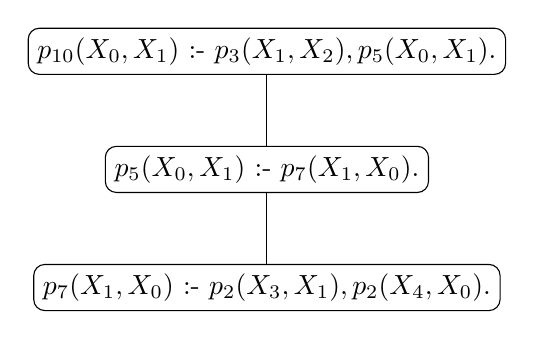
\begin{tikzpicture}[sibling distance=10em,every node/.style = {shape=rectangle, rounded corners, draw, align=center, top color=white}]]%, bottom color=blue!20
            \node {$p_{10}(X_0,X_1) \ass {p_3(X_1,X_2)},p_{5}(X_0,X_1).$}
            child { node {$%\mathbf
            {p_{5}(X_0,X_1)}\ass {p_{7}(X_1,X_0)}.$} edge from parent%[->]
            child { node {$%\mathbf
            {p_{7}(X_1,X_0)} \ass p_2(X_3,X_1),p_{2}(X_4,X_0).$} edge from parent%[->]
            } };
        \end{tikzpicture}}
       }
%   
%  |- [0] p6(X0,X1) :- p3(X2,X1),p2(X0,X2).
% 	|- [1] p3(X2,X1) :- p4(X2,X1).
% 		|- [3] p4(X2,X1) :- p10(X2,X1).
% 	|- [2] p2(X0,X2) :- p7(X2,X0).
% 		|- [4] p7(X2,X0) :- p8(X2,X0).
  \subfigure[Rooted DG]{
        \centering
        \fbox{
        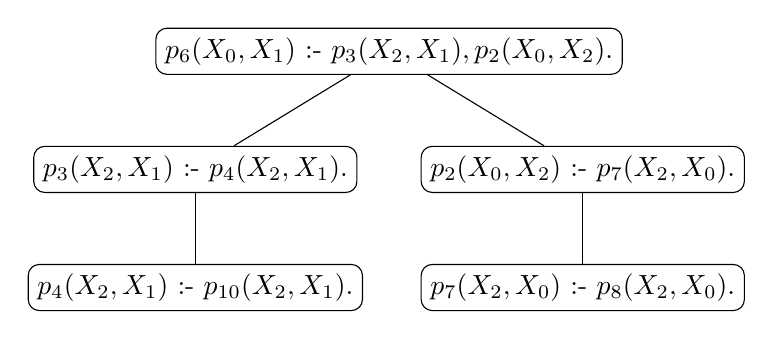
\begin{tikzpicture}[sibling distance=14em,
        every node/.style = {shape=rectangle, rounded corners,
        draw, align=center,
        top color=white}]]%, bottom color=blue!20
            \node {$p_6(X_0,X_1) \ass p_3(X_2,X_1),p_2(X_0,X_2).$}
            child { node {$p_3(X_2,X_1) \ass p_4(X_2,X_1).$} 
            child { node {$p_{4}(X_2,X_1) \ass p_{10}(X_2,X_1).$}}}
            child { node {$p_2(X_0,X_2) \ass p_7(X_2,X_0).$}
            child { node {$p_{7}(X_2,X_0) \ass p_{8}(X_2,X_0).$}}};
        \end{tikzpicture}}
    }
    % 
%      |- [0] p2(X0,X1) :- p6(X0,X1).
% 	|- [1] p6(X0,X1) :- p4(X2,X0),p8(X0,X1).
% 		|- [2] OR
% 			|- [3] p4(X2,X0) :- p4(X0,X3),p3(X2).
% 			|- [4] p4(X2,X0) :- p3(X0),p9(X2,X0).
    \subfigure[Disjunctive Rooted DG]{
        \centering
        \fbox{
        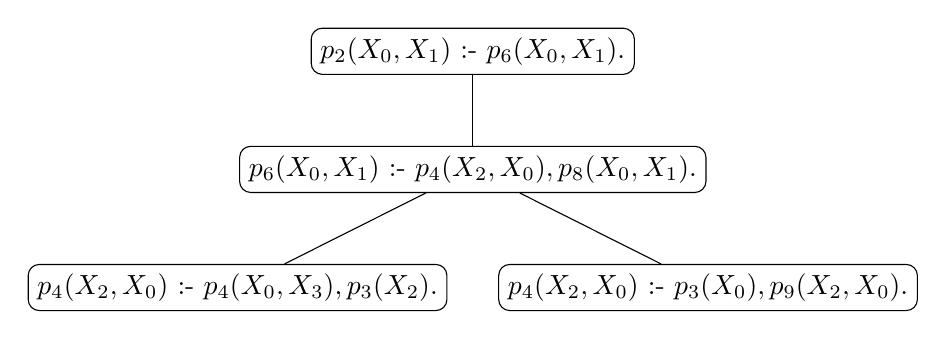
\begin{tikzpicture}[sibling distance=17em,
        every node/.style = {shape=rectangle, rounded corners,
        draw, align=center,
        top color=white}]]%, bottom color=blue!20
            \node {$p_2(X_0,X_1) \ass p_6(X_0,X_1).$}
            child { node {$p_6(X_0,X_1) \ass p_4(X_2,X_0),p_8(X_0,X_1).$} 
           % child[node distance=0.01mm] { node[node distance=0.01mm]{}
            % %
            child { node {$p_4(X_2,X_0) \ass p_4(X_0,X_3),p_3(X_2).$} }
             child { node {$p_4(X_2,X_0) \ass p_3(X_0),p_9(X_2,X_0).$}}        %}
             };
        \end{tikzpicture}}
    }
    \caption{Example rule sets generated for the different categories (the rules of datasets
    (a) CHAIN-S, (b) RDG-S, (c) DRDG-XS).}
    % Categories (a) Chain, (b) Rooted DG, and (c) Disjunctive Rooted DG}
    \label{fig:datasets}
\end{figure*}



% \begin{figure}
% \centering
% % |- [0] p0(X0,X1) :- p3(X1),p18(X0).
% %  |- [1] p18(X0) :- p15(X0,c46).
% %   |- [2] p15(X0,X2) :- p4(X2),p11(X0).
% \fbox{
% \begin{tikzpicture}[sibling distance=10em,
% every node/.style = {shape=rectangle, rounded corners,
% draw, align=center,
% top color=white}]]%, bottom color=blue!20
% \node {$p_0(X_0,X_1) \ass p_3(X_1),p_{18}(X_0)$}
% child { node {$p_{18}(X_0) \ass p_{15}(X_0,c_{46})$} edge from parent[->]
% child { node {$p_{15}(X_0,X_1) \ass p_4(X_1),p_{11}(X_0)$} edge from parent[->]} };
% \end{tikzpicture}}
% % - [0] p0(X0,X1) :- p6(X1,X2),p5(X0).
% %  |- [1] OR
% %   |- [2] p5(X0) :- p8(X0,X0).
% %   |- [4] p8(X0,X0) :- p16(X0).
% %   |- [3] p5(X0) :- p7(X0).
% %   |- [5] p7(X0) :- p19(X0).
% \fbox{
% \begin{tikzpicture}[sibling distance=10em,
% every node/.style = {shape=rectangle, rounded corners,
% draw, align=center,
% top color=white}]]%, bottom color=blue!20
% \node {$p_0(X_0,X_1) \ass p_6(X_1,X_2),p_5(X_0)$}
% child { node {$p_5(X_0) \ass p_8(X_0,X_0)$} 
% child { node {$p_8(X_0,X_0) \ass p_{16}(X_0)$}}}
% %
% child { node {$p_5(X_0) \ass p_7(X_0)$} 
% child { node {$p_7(X_0) \ass p_{19}(X_0)$}}};
% \end{tikzpicture}}
% \caption{Rule sets generated for Categories Chain, Rooted DAG, and Disjunctive Rooted DAG}
% \label{fig:datasets}
% \end{figure}



\begin{table*}[h!]
    \centering
    \begin{tabular}{|l|l|l|c|c|c|c|c|}
    \hline
     Name & Size & Category   & \#Facts&\#Rules & \#Predicates & \#Constants \\%& Depth of  \\
          % &  & Category &&&&\\%& Rule Graph \\
     \hline
     CHAIN-XS & tiny & Chain &64 &3& 9&  37\\% size, 64 , predicates, 9 , constants, 37
     RDG-XS & tiny & R-DG & 93& 4&8 &42 \\%train: size, 93 , predicates, 8 , constants, 42
     DRDG-XS & tiny & DR-DG &76 &4& 11&34 \\%size, 76 , predicates, 11 , constants, 34
     CHAIN-S & small & Chain &572 &3& 11 &205 \\% size, 572 , predicates, 11 , constants, 205
     RDG-S & small & R-DG &375 &5 &11&215  \\%\textbf{train: size, 357 , predicates, 11 , constants, 215}
     DRDG-S & small & DR-DG &945 &6&11 &  406\\\hline%size, 945 , predicates, 11 , constants, 406
    \end{tabular}
    \caption{Overview of our generated datasets; all rule graphs have depth three.}
    \label{tab:datasets}
\end{table*}

We have generated several example datasets that reflect different possible scenarios. Specifically, they vary in the sorts and quantity of facts and in the structures and sizes of the rule sets (example rule sets are depicted in Figure~\ref{fig:datasets}).
Each dataset consists of two files, one for the facts and one for the rules,
both come in standard Prolog format. 
%
The datasets described in this section were generated under the open-world assumption. Specifically,  %That is, the sets facts do not necessarily contain all facts that are true in the corresponding scenario. In fact, 
we configured the generator such that they contain only 70\% of the consequences that can be inferred from a basic set of so-called \emph{\support facts} (this is detailed in Section~\ref{sec:generation}).

\textbf{Rules and facts.}
Our datasets are domain independent, which means that we consider synthetic names $p_i$ for %\emph #VERONIKA: introduce in previous section!
{predicates}, $c_i$ for {constants}, and $X_i$ for {variables} with $i\ge0$. %$p_0$ is the \textit{target predicate}.
% 
We generate datalog \emph{rules} as introduced in Section~\ref{sec:motivation}.
% \begin{equation}\label{eq:rule}
%     \alpha_0\ass\alpha_1,\dots,\alpha_m .
% \end{equation}
% of length $m\ge1$ where all %\emph
% {atoms} $\alpha_j$, $0\le j\le m$, are of the form $p(t_1,\dots,t_n)$ with a predicate $p$ of arity $n\ge1$ and terms $t_k$, $1\le k\le n$.
% A %\emph
% {term} is either a constant or a variable. 
% $\alpha_0$ is called the %\emph
% {head} and the conjunction $\alpha_1,\dots,\alpha_m$ the %\emph
% {body} of the rule. All variables that occur in the head must occur in the body.
% 
For practicality, we require the head to contain some variable, and set both the maximum rule length and arity of atoms to two (these are parameters configurable in the generator).
% % 
% Note that these rules are similar but more general than the rules considered in related work. More specifically, we do not require dependencies between the variables in the body (e.g., closed paths) and
%we neither restrict the predicates to be binary and the rule length to be two nor require dependencies between the variables in the body (e.g., closed paths). Furthermore, we 
% allow the rules to contain constants and to be recursive; that is, the predicate occurring in the head atom may also occur in body atoms.
%
% A \emph{fact} is an atom that does not contain variables.

We divide rule sets into three different categories depending on the dependencies between rules: \emph{Chain}, \emph{Rooted DG}, and \emph{Disjunctive Rooted DG}; and generated complete datasets for each. %, Mixed}.  %rule sets (or rather, complete datasets) for eac.
Figure~\ref{fig:datasets} shows the generated rule sets. % for each category. 
The dependencies between the rules are represented as edges in a directed graph (DG) where the rules are the nodes. That is, an incoming edge at a node shows that the facts inferred by this rule might be relevant for inference with the rule at the connected node.
The %rule at the top is used to infer the \emph{target} facts and the corresponding node
node at the top
is called the \emph{root}. In the following, we use (rule) graph and DG interchangeably. %and may sometimes directly refer to the graph when 

\textbf{Category Chain.} Each rule apart from the one at the root infers facts relevant for exactly one other rule (i.e., every node has at most one parent node) and, for each rule, there is at most one such other rule which might infer facts relevant for the rule (i.e., every node has at most one child node). However, recursive rules represent an exception, they are relevant for themselves and for one other rule (i.e., the graph has a small loop at each node representing a recursive rule).
% 

\textbf{Category Rooted DG.} It generalizes category Chain in that every rule can be relevant for several others (i.e., every node has at most one parent node).
Furthermore, for each rule, there may be several other rules which might infer facts relevant for the rule (i.e., a node may have several child nodes). However, for each predicate occurring in the body of the former rule, there must be at most one other rule with this predicate in the head; %or the predicate also occurs multiple times in body (in case several parent situation is converted to fact graph) - MENTION THIS EXCEPTION HERE
that is, there are no alternative rules to derive facts relevant for a rule w.r.t.\ a specific body atom. 
%

\textbf{Category Disjunctive Rooted DG.} It generalizes category Rooted DG in that we do not have the restriction regarding the latter alternatives.

Figure~\ref{fig:datasets} illustrates the differences between the categories. In (a), for every rule, there is at most one child node with a rule relevant for its derivations.
In (b), there might be multiple, but the child nodes contain different predicates in their heads. In (c), the latter does not hold anymore. That is, for given facts, there may be alternative derivations leading to positive examples.

Table~\ref{tab:datasets} shows statistics about the datasets we generated.
Observe that, in addition to the datasets whose rules are shown in Figure~\ref{fig:datasets}, we present one larger dataset for each category.
The dataset size describes the dimension of the fact sets.
All the datasets were generated such that they are missing 30\% of all consequences,  20\% of the original support facts, and contain 20\% facts that are irrelevant for the derivation of positive examples. We hence simulated an open-world setting and considered noise.
Observe that, in terms of size, these datasets are comparable to existing most ones such as .... We also generated corresponding datasets where all rule graphs have depth two; and we have larger datasets, but the results ... (see Section~\ref{sec:experiments}).

\veronika{complete %figure (add rule sets of finally generated datasets), tab, and 
above explanation, mention pred nbrs, comment on difficulty - first want to show that even simple rules learned in other papers in combination tricky see c, mention var indexes, or node}
% \veronika{we have also versions for depth 2 but maybe that would be overwhelming, .  }


% \veronika{scalable is a system property rather than one of the datasets, no? maybe call it dimension:small/large? or use medium/large and say that we call small sth like Evans. and we can extend it in the future to XL etc. ;)}
% \veronika{I would use names that are easy to use as file names (so without subscripts) therefore I changed it. we can also use other names still...}
% \veronika{I did not mention recursion here as specific category but would include it into every of the others (ie. we here just take the recursive version we have for all in the code }
% \veronika{maybe RDG instead of R-DG etc. but I do not have a strong opinion on that }

% \veronika{I try to not use target predicate or facts since %p0 = target predicate can we say this although 
% basically we have a kind of target predicate with every rule... however I would find it better, given the rule catgories and dependencies, to talk about p0 as target predicate and the corrsponding atoms as positive and negative examples (as in standard ILP problems) rather than to consider them for each rule. what do you think?}
% recursion -> h(X):-h(Y),b1(X,Y). b1(X,Y):-b1(Z,Y),b2(X,Z)
% rooted DAGs -> h:-b1,b2. b1:-a1,a2. b2:-c1,c2. a1:-d1,d2. a2:-d3,d4. ...
% rooted DAGs + OR -> different rules same head: h:-b1,b2. h:-a1,a2. h:-c1,c2.
% chains -> h:-b1,b2. b1:-a1,a2. a1:-c1,c2
% mix -> expecially for training

% \veronika{I think until now I never use 'root' anywhere}
\section{Dataset Generation}\label{sec:generation}
%\veronika{describe how we generated the different configurations }
% \veronika{list the cases we exclude in the generation (e.g., rules with only constants in head) to show that the generation is not that easy?}
%what we need/have is safety etc. not only constants in head
% or are this properties of the datasets rather?

\tool contains an easy-to-use generator of ILP datasets 
as %the ones 
presented in Section~\ref{sec:description}. 
It is written in Python. In this section, we describe the generation of the rules and facts in detail.
%It first determines the arity of the predicates considered randomly and then generates the rules and corresponding facts. Note that, in addition to the set of facts generated under the open-world assumption, it also generates a closed-world version of the fact set.
% It produces a 

\textbf{Configuration.} \tool is parameterizable in many dimensions, most important are the following:
\begin{itemize}
\item maximal number of predicates and constants
\item maximal arity of predicates
\item dataset size: XS, S, M, L, XL
%  XS = (50, 100, 3)
%     S = (101, 1000, 5)
%     M = (1001,10000, 10)
%     L = (10001, 100000, 20)
%     XL = (100001, 500000, 50)
\item open-world degree \nowa (percentage) % $n_O$)
\item amount of noise in the data \nnoise (percentage) % $n_N$)
\item minimal and maximal number of DGs in the rule set
\item category of DGs: Chain, R-DG, DR-DG, Mixed
\item number and maximal length of rules
\item maximal depth of rule graphs
\end{itemize}
Observe that the latter is a bound for the number of inference steps, and that the number of available predicates and constants influences the variability and number of generated facts, rules, and noise.
An XS dataset contains about 50-100 facts, 
an S dataset about 101-1,000, 
an M dataset about 1,001-10,000,
an L dataset about 10,001-100,000,
and an XL dataset about 100,001-500,000. Note that \tool can easily be extended to allow for new sizes like XXL, etc.
The open-world degree specifies how many of the consequences from a basic set of {\support facts} are missing in the dataset,
and the amount of noise determines how many \support facts are missing and how many facts irrelevant for deriving the target facts are contained in the dataset.
By number of DGs in a rule set, we mean the number of connected components in the graph of a rule set, where the rules are considered as nodes in a graph and the edges represent the dependencies between them (see Figure~\ref{fig:datasets}).
Category mixed specifies that these connected components may be of different categories.
% In the following, we describe 
The implementation of a given configuration is described in detail in the following.
% A more detailed description of these two degrees is 
%Specifically, we divide the set of consequences into target facts and remaining consequences and remove $n_{OWA}$\% of both from the dataset.
%The amount of noise determines the amount of data that is removed from the \support facts and replaced by arbitrary facts that are irrelevant for the derivation of the target facts. We also add a corresponding number of noise to the set of target facts (i.e., ).

\textbf{Preprocessing.}
The number of DGs that is being generated and their depths are determined randomly; though, we ensure that at least one graph is of the given maximal depth.
Note that all random selections we mention are within the bounds given in the configuration under consideration.
% Then, if not specified in the configuration, 
% the necessary numbers of predicates and constants are computed based on the other parameters in the configuration (e.g., requested dataset size, \nowa, etc.).
Also the arities of the predicates are selected at arbitrarily. 
Predicates are named ${p_0},p_1,\dots$ and constants $c_0,c_1,\dots$.
%and the number and size.
%It first determines the arity of the predicates considered randomly and then generates the rules and corresponding facts. Note that, in addition to the set of facts generated under the open-world assumption, it also generates a closed-world version of the fact set.
% It produces a 

\textbf{Rule generation.}
According to the rule set category specified and graph depths determined, rules (nodes in the graph) of form (\ref{eq:rule}) are generated top down breadth first, for each of the rule graphs to be constructed. 
The generation is largely at random, that is, w.r.t.
the number of child nodes of a node and which body atom they relate to, respectively; 
the number of atoms in a rule; and the predicates within the latter, including the choice of the target predicate in the very first step. Though, \tool also offers the option that all graphs have the same target predicate.
% 
In order to allow for more derivations, we currently only consider variables as terms in head atoms; the choice of the remaining terms is based on probabilities as described in the following. 
% as follows. 
Given the atoms to be considered (in terms of their number and predicates) and an arbitrary choice of head variables, we first determine a position for each of the latter in the former. Then we populate the other positions one after the other: a head variable is chosen with probability $0.2$ ($[1/5]$); for one of the variables introduced so far, we have probability $0.6$ ($[4/5] * [3/4]$); for a constant, $0.02$ ($[4/5] * [1/4] * [1/10]$); and, for a fresh variable, $0.18$ ($[4/5] * [1/4] * [9/10]$); note that the probabilities can be changed easily.

\textbf{Fact generation.}
The fact generation is done in three phases: we first construct a set \db of relevant facts in a closed-world setting, consisting of {\support facts} \sfacts and their {consequences} \cfacts, and then adapt it according to \nowa and \nnoise.
% then delete some consequences according to \nowa, %the specified open-world degree, 
% and lastly create noise by deleting \support facts and adding arbitrary facts according to~\nnoise.
% Based on the assumption that ILP systems need positive examples for a rule to learn that rule, we consider, for each rule of form (\ref{eq:rule}), $n_B$ different variable assignments and, for each assignment $\sigma$, generate the facts $\sigma(\alpha_0),\sigma(\alpha_1),\dots,\sigma(\alpha_m)$.
% We call the resulting set \emph{base facts}. $n_B$ depends on the dataset size specified: we set $n_B=3$ for small datasets, $n_B=X$ for medium datasets, and $n_B=Y$ for large datasets.

The (natural) idea is to generate facts by instantiating the rule graphs multiple times,
based on the assumption that ILP systems need positive examples for a rule to learn that rule, and to stop the generation when the requested number of facts has been generated. Though, we actually stop later because we need to account for the fact that we subsequently will delete some of them % consequences 
according to \nowa. 
%TODO Also note that recursive rules cannot lead to an unexpectedly large dataset because the variables in the rule heads occur in the body. 
%\veronika{more proof needed! see comments file}
% and, more importantly, we do not have existential - VERONIKA don't think we do have to mention this since we do not consider existentials at all in the paper
%Specifically, for each rule of form (\ref{eq:rule}), $n_B$ different variable assignments and, for each assignment $\sigma$, generate the facts $\sigma(\alpha_0),\sigma(\alpha_1),\dots,\sigma(\alpha_m)$.
%In detail, the process is as follows. We 
More specifically, we continuously iterate over all rule graphs, for each, select an arbitrary but fresh variable assignment $\sigma$, and then iterate over the graph nodes as described in the following, in a bottom-up way. 
% 
% The remaining relevant facts, \emph{support facts} and \emph{consequences}, are constructed as follows.
% We consider $n_S$ different variable assignments and, for each assignment $\sigma$,
% iterate over the nodes in the rule graph in a bottom-up way. %, maintaining a list of processed nodes.
First, we consider each leaf $n$ and corresponding rule of form (\ref{eq:rule}) %add $n$ to the processed nodes, 
and generate support facts $\sigma(\alpha_1),\dots,\sigma(\alpha_m)$.
Then, we infer the consequences based on the rules and all facts generated so far. %(i.e., including the base facts).
For every node $n$ on the next level and corresponding rule of form (\ref{eq:rule}), we only generate those of the facts $\sigma(\alpha_1),\dots,\sigma(\alpha_m)$ as support facts which are not among the consequences inferred previously. We then again apply inference, possibly obtaining new consequences, and continue iterating over all nodes in the graph in this way.
%$n_S$ ...
%TODO consider node only in 60% probab  ie ignore with30
We further diversify the process based on two integer parameters, \ndag and \nnskip: in every \ndag-th iteration the graph is instantiated exactly in the way  described; in the other iterations, we skip the instantiation of a node with probability 1/\nnskip and, in the case of DR-DGs, only instantiate a single branch below disjunctive nodes. %in the imokementation actually 1/(n+1)

In the open-world setting, we subsequently construct a set \dbowa by randomly deleting consequences from \db according to the open-world degree given: 
assuming $\tfacts\subseteq\cfacts$ to be the set of target facts, 
we remove $\nowa\%$ from $\cfacts\setminus\tfacts$, and similarly $\nowa\%$ from \tfacts.
In this way, we ensure that the open-world degree is reflected in the target facts. Though, note that there is the option to have it more arbitrary by removing $\nowa\%$ from $\cfacts$ instead of splitting the deletion into two parts.
% $\cfacts_{\text{R}}$
% % assuming \db to be the set of generated facts and $\targets\subseteq\db$ to be the set of target facts, 
% we remove $\nowa\%$ from $\db\setminus\targets$, but only consequences, and similarly $\nowa\%$ from \targets.

The noise generation is split similarly and focuses on two kinds of noise, missing and irrelevant facts. %
Specifically, we construct a set \dbowan based on \dbowa by arbitrarily removing $\nnoise\%$ from \sfacts, and by adding arbitrary fresh facts that are neither in \cfacts (i.e., we do not add facts which we have removed in the previous step) nor contain the target predicate
such that $\dbowan\setminus\tfacts$ contains $\nnoise\%$ of noise.
% The number of the latter facts we remove %and add 
% amounts to $\nnoise\%$ of \sfacts; we %$\nnoise\%$ of $\dbowa\setminus\tfacts$, respectively.
In addition, we add arbitrary fresh facts containing the target predicate and that are neither in \tfacts %ie also not removed in owa part
such that the set of facts within \dbowan on that predicate finally contains $\nnoise\%$ of noise.

 
% For the first, some of the relevant facts are removed randomly. We however must not remove facts that were added in the inference steps before in the closed-world setting to maintain the closed-world assumption (i.e., there, we do not delete consequences), and never delete base facts.
% % (i.e., we do not delete consequences, which include all target atoms).
% Regarding the second kind of noise, arbitrary facts are added. Note that we also add facts on predicates that occur in rule heads as negative examples in both the open- and the closed-world setting.
% In the latter, we again apply inference afterwards such that the resulting fact set also contains the consequences of the added noise to satisfy the closed-world assumption.
% As a result, the generator produces a dataset that contains the amount of noise specified %$n_N$\% noise 
% in both the facts on $p_0$ and in the remaining facts.


\textbf{Output.}
The dataset generation produces the following:
\begin{itemize}
\item The rules and a \emph{training} set (\dbowan) which, is of the requested size, and fulfills \nowa and \nnoise.
\item A \emph{validation} and a \emph{test} set as required by most of the current systems containing the consequences which were removed from the original, closed-world version \db using a split of 1:2. 
% \item Files containing the predicates and constants occurring in \db.
%For these systems \GER also provides the predicates and constants occurring in \db.
%\item \db, an adaptation of that set which contains noise (but all of \cfacts), \sfacts, and 
%\cfacts~ -- for further experiments.
\item %Finally, for evaluation purposes in our generator, we generate a set of facts  
% A set $\db'$ of facts generated in the same way as \db and use the \support facts of that set as a custom 
A custom \emph{evaluation} set $\sfacts'$ for our evaluation tools that is
generated in the same way as \sfacts.
\veronika{still open if we need it for our evaluation, if not remove here}
% \item 
% For further experiments, \tool actually 
% also outputs 
% \db, an adaptation of that set which contains noise (but all of \cfacts), \dbowa, \sfacts, \cfacts, and files containing the predicates and constants occurring in \db.
\end{itemize}
For further experiments, \tool actually 
also writes out
\db, an adaptation of that set which contains noise (but all of \cfacts), \dbowa, \sfacts, \cfacts, and files containing the predicates and constants occurring in \db.
%is in previous section already: All files are in Prolog syntax.
% a set of rules and a \emph{training} set, which contains the set \dbowan, is of the requested size, and fulfills \nowa and \nnoise. The consequences which were removed from the original, closed-world version \db are used to produce a \emph{validation} and a \emph{test} set as required by most of the current systems using a split of 1:2. %\footnote{Traditionally, the rules are not available for evaluation } 
% For further experiments, \tool also provides %the original, closed-world version of 
% \db, an adaptation of that set which contains noise (but all of \cfacts), \sfacts, and 
% \cfacts.
% %
% Finally, for evaluation purposes in our generator, we generate a set of facts $\db'$ in the same way as \db and use the \support facts of that set as a custom \emph{evaluation} set for our evaluation tools. 

%\veronika{should we directly output a set of negative examples too? it can be easily constructed though, from \tfacts using all constants occurring in \db. maybe yes because we talk about ILP datasets in the beginning of the section -- or delete ILP there?}

% files in Prolog syntax:
% \begin{itemize}
% \item \fi{rules}: the rule set
% \item \fi{train}: the dataset of 
% \end{itemize}

% \veronika{need to think about how we describe parts as the one in the comment below. can you call this "conditioning"? I guess I have to calculate the percentages from that}
%   args = [ hvs[hvps.index((j,p.name, i))] if (j,p.name, i) in hvps 
%else hvs[random.randint(0, len(hvs)-1)] if random.randint(0, 5) == 0
%else allvars[random.randint(0, len(allvars)-1)] if allvars != [] and random.randint(0, 2) == 0
% else constants[random.randint(0, len(constants)-1)] if random.randint(0, 1) == 0
%              else self.get_new_var() 
%              for i in range(p.arity)]
%  \veronika{we also plan to do sometimes depth first rule generation. can we describe here already that we have done it mixed and implement it for camera ready? not sure}
%  \veronika{currently, I do a category check in the end and if it's a chain but we want an RDG I regenerate. but that's not so nice so maybe just drop this here?}


% \veronika{decide about $n_B$. makes sense in dependence of size, no? (latter is better than making it a parameter, no? ) best would be if it also depends on max reasoning depth mabybe? what do you think? and how?}
% \veronika{I do not understand the following: \\predicate invention: we don't want them in the dataset and rules:
% we don't want to have auxiliary predicates in the dataset
% having them would imply that the theory can be expressed using binary rules and so we will not need predicate invention in our system
% we could just eliminate them from the facts but since the dataset is automatically generated, we can not distinguish them from the name compared to normal predicate 
% }
% \cristina{This is for the evaluation, and not for the generation}
% \veronika{number of reasoning steps - we cannot control that since rules can be applied recursively sometimes or iteratively in loops. therefore I used max grpah depth}
% \veronika{}
% \veronika{I added size of fact set since nbr of facts is hardly controllable because of inference. (ok, we could always delete consequences but I am not sure, what do you think? or use max num facts?) we also have to think about how to make sure the generated datasets is corresponding. maybe check after generation and otherwise regenerate. eg in case inference surprisingly lead to 1000 more facts}

% \veronika{in intro: variable assignment}
% \veronika{in cwa we can hardly control dataset size. should we say that it applies to owa? or do you have an idea?}
% \veronika{one might make a figure with the generation of the the relevant facts but I am not sure if this is necessary or the text is understandable. or/and better add an example?}


% \textbf{Test Set.}
% \cristina{Describe random generation of testing set and homogeneous generation}
\section{Evaluation Tools}
\label{sec:evaluation}
\veronika{introduce preliminaries specific for measures here. they are not needed if you just read the paper to learn about the datasets...}

Evaluation tool to compute distances between logic programs:
 There are 2 (or more) types  of distances defined on logic programs
\begin{itemize}
    \item  distance between Herbrand interpretations 
    \item directly on rules (logic programs)  
\end{itemize}

we don't count auxiliary pred

the distances can be considered ``fuzzy'' in the sense that we consider facts with weights

\veronika{I think we should also compute measures they considered so far - like Hits@... AUC , ... -- and the discuss how the results vary}
\section{Experiments}\label{sec:experiments}


\begin{table*}[h!]
    \centering
    \begin{tabular}{|l|l|l|c|c|c|c|c|}
    \hline
     Name & Size & Category   & \#Facts&\#Rules & \#Predicates & \#Constants \\%& Depth of  \\
          % &  & Category &&&&\\%& Rule Graph \\
     \hline
     CHAIN-XS & tiny & Chain &76&2&9&51\\%train: size, 76 , predicates, 9 , constants, 51
     RDG-XS & tiny & R-DG &63&3&9&35  \\%train: size, 63 , predicates, 9 , constants, 35
     DRDG-XS & tiny & DR-DG & 97&3&11 &67 \\%size, 97 , predicates, 11 , constants, 67
     CHAIN-S & small & Chain & 677&2& 11 & 287\\%size, 677 , predicates, 11 , constants, 287
     RDG-S & small & R-DG &634&3&11& 379 \\%size, 634 , predicates, 11 , constants, 379
     DRDG-S & small & DR-DG & 790&3&11 &  301\\\hline%ize, 790 , predicates, 11 , constants, 301
    \end{tabular}
    \caption{Overview of generated datasets with rule graphs of depth two.}
    \label{tab:datasets2}
\end{table*}


\begin{table*}[t!]
    \centering
    \begin{tabular}{|l|c|c|c|c|c|c|c|}
    \hline
    %  Name & Size & Rules   & \#Facts&\#Rules & \#Predicates & \#Constants & Depth of  \\
    %       &  & Category &&&&& Rule Graph \\
    %  \hline
     &  EVEN & S-2-1 N &  S-2-2 N &  XS-1 N &  S-2-1 E &  S-2-2 E &  XS-1 E \\\hline
     FOIL & \bf{1.0} & 0.0052 [\bf{1.0}] & 0.0 & 0.0 & 0.575 [\bf{0.982}] &0.0333 [\bf{1.0}] & \bf{0.816} [\bf{1.0}] \\\hline
     Amie  & - & \bf{0.955} & \bf{1.0} & 0.7029& \bf{0.955} & \bf{0.714} & 0.7029 \\\hline
     Neural LP  & - & 0.0 & 0.0 & 0.234  & 0.0 & 0.0& 0.7029 \\\hline
     NTP  & \bf{1.0} & 0.382 &0.03 & \bf{1.0} & 0.382 &0.031 & 0.0 \\\hline
    \end{tabular}
    \caption{\centering Herbrand accuracy for simple datasets (CHAIN). \\ Standard confidence is reported in parenthesis when different from Herbrand accuracy.}
    \label{tab:results}
\end{table*}

%\begin{table*}[t!]
%    \centering
%    \begin{tabular}{|l|c|c|c|c|c|c|c|}
%    \hline
%     &   EVEN & S-2-1 N &  S-2-2 N &  XS-1 N &  S-2-1 E &  S-2-2 E &  XS-1 E \\\hline
%     FOIL  & \bf{1.0} & \bf{1.0} & 0.0 & 0.0&  \bf{0.982} & \bf{1.0} & \bf{1.0}  \\\hline
%     Amie & - & 0.955 & \bf{1.0} & 0.7029 & 0.955 &0.714 & 0.7029 \\\hline
%     Neural LP & - & 0.0 & 0.0 &0.234 &0.0 & 0.0 & 0.7029 \\\hline
%     NTP & \bf{1.0} &0.382 & 0.03& \bf{1.0} & 0.382& 0.031& 0.0  \\\hline
%    \end{tabular}
%    \caption{Standard confidence for simple and existing datasets (CHAIN)}
%    \label{tab:results}
%\end{table*}

\begin{table*}[t!]
    \centering
    \begin{tabular}{|l|c|c|c|c|}
    \hline
     &  CHAIN-S-2 & CHAIN-S-2-0 &  CHAIN-S-3 &  CHAIN-XS-2 \\\hline
     FOIL & 0.608 [\bf{0.954}] & 0.354 [0.784] & 0.654 [\bf{0.958}] & 0.329 [0.350] \\\hline
     Amie & \bf{0.6262} & \bf{0.6981} & \bf{0.8860} & \bf{0.8667} \\\hline
     Neural LP & 0.0021 [0.0022] & 0.0 & 0.0312 [0.0318]& 0.0533\\\hline
     NTP  &0.0 & 0.0064 & 0.0225 [0.0256] & 0.1610 [0.1755] \\\hline
    \end{tabular}
    \caption{\centering Herbrand accuracy for binary datasets (CHAIN)\\ Standard confidence is reported in parentesis when different from Herbrand accuracy.}
    \label{tab:results}
\end{table*}


\begin{table*}[t!]
    \centering
    \begin{tabular}{|l|c|c|c|c|c|c|}
    \hline
     &  DRDG-S-2 &  DRDG-S-3 &  DRDG-XS-2 & RDG-S-2 & RDG-S-3 & RDG-XS-2\\\hline
     FOIL &0.193 [0.783] & 0.0 & \bf{0.703} [\bf{0.734}] & 0.0 & 0.515 [\bf{0.911}]& \bf{0.496} [\bf{0.624}] \\\hline
     Amie  &  & \bf{0.4898} & 0.0064 & \bf{0.7137} & & 0.2208 \\\hline
     Neural LP & 0.0080 [0.0083]& 0.0816 [0.0857] &0.0649 [0.0671] & 0.0741 [0.0831] & 0.0482 [0.07958] &0.0029 [0.0031] \\\hline
     NTP & & 0.1801 [0.2068]& 0.1236 & 0.1429 & 0.0 &0.0073\\\hline
    \end{tabular}
    \caption{\centering Herbrand accuracy for binary datasets (DRDG and RDG)\\ Standard confidence is reported in parentesis when different from Herbrand accuracy.}
    \label{tab:results}
\end{table*}

We ran experiments with representatives of the different types of rule learning systems using the datasets described in Section~\ref{sec:description}. In this section, we report and discuss the results.

\subsection{Systems}
We evaluated the following systems.

\textbf{FOIL.} \cite{Quinlan-ML90:foil}
A traditional ILP system whose rule construction is completely driven by positive and negative examples in that the rule bodies are iteratively refined (i.e., atoms are added) until none of the negative examples can be derived by the rule anymore -- though exceptions are possible. The process is guided by custom heuristics based on the examples.
% : after the selection of the head atom, body atoms are iteratively added until none of the negative examples
%progol:
% It combines \emph{inverse entailment} 
% with general-to-specific search through a refinement graph. 
% % Inverse Entailment is used with mode declarations to derive the most-specific clause within the mode language which entails a given example. This clause is used to guide a refinement-graph search. Unlike the searches of Shapiro's MIS and Quinlan's FOIL, Progol's search is efficient and has a 
% The search has been proven to return a solution having the maximum "compression" in the search-space. 
% \veronika{explain Inverse Entailment and compression}
% \veronika{alternatively use FOIL. I think one of the old approaches where we probably get not too strong results is enough because there is not really a point to running `bad' systems, no?}

\textbf{AMIE+.} \cite{Galarraga+-VLDBJ15:amiep} A system mining rules systematically by considering rules with a single body atom and then iteratively refining them %by adding body atoms 
based on custom confidence and coverage measures.
For medium-sized KBs, it has been shown to be several orders of magnitude faster than other state-of-the-art systems. 
%We use the preconfigured parameters but set .. in order
% \veronika{sketch approach} mention converage confidence refinement, pruning

% AMIE also requires the rules to be closed. A variable in a rule is closed if it appears at least twice
% in the rule. A rule is closed if all its variables are
% closed. The restriction to closed rules avoids mining
% rules that predict merely the existence of a fact, as in
% diedIn(x, y) ⇒ ∃z : wasBornIn(x, z).
% AMIE omits also reflexive rules, i.e., rules with

\textbf{Neural LP.} \cite{YaYaCo-NIPS17:neurallp} One of the first end-to-end differentiable approaches. 
\veronika{one sentence about processing (matrix multiplication?). I do not fully understand it, find the description somehow vague "based on tensorlog"..}
Neural LP is special in that it learns
a distribution over logical rules, instead of
an approximation to a particular rule, such that its inference is based on rules that have these confidences attached as weights.


% , and this distributiom During
% inference time.

\textbf{NTP.} \cite{RoR-NIPS17} Similarly, a recent neural approach that recursively constructs a network which derives the training examples through backward chaining.
It is based on learning vector embeddings of symbols and represents symbolic unification by computationally combining them.
%based on using embeddings for ... 
%\veronika{evaluate one traditional ILP system and the neural approaches we get hold of}
%riedel
%mention that we did not get hold of the other systems
%Complex[7] as link prediction approach?
%As NTPs can learn rules from data, they are related to ILP systems such as FOIL [32], Sherlock [57] and meta-interpretive learning of higher-order dyadic Datalog (Metagol) [58]. While these ILP systems operate on symbols and search over the discrete space of logical rules, NTPs work with subsymbolic representations and induce rules using gradient descent. 
%Recently, [37] introduced a differentiable rule learning system based on TensorLog and a neural network controller similar to LSTMs 

\veronika{neural lp:is `one of the first' true?} 

\veronika{FOIL: I only coarsely read the paper and did not find the point where it describes which head predicates are considered for rule construction. all possible ones? it says it starts with the target predicate}

\subsection{Implementation}
We ran all systems on the same machine, a ...

\veronika{mention specific configuration params we use with below links?} 
FOIL\footnote{\url{http://www.cs.cmu.edu/afs/cs/project/ai-repository-9/ai/util/areas/learning/systems/foil/foil5/0.html}} (version 5)
AMIE+\footnote{\url{https://www.mpi-inf.mpg.de/departments/databases-and-information-systems/research/yago-naga/amie/}} (version of 2015-08-26)
And code of following (current date)...
Neural LP\footnote{\url{https://github.com/fanyangxyz/Neural-LP}}
NTP\footnote{\url{https://github.com/uclmr/ntp}}
The scripts for running the evaluation are available in our GitHub repository.

\veronika{mention negative examples given to FOIL and how we handle validation facts for ntp... and in general}

Since Neural LP and AMIE+ only support binary atoms, we represent unary atoms of forms $p(X)$ and $p(c)$ by $p(X,X)$ and $p(c,c)$, respectively, as it is usual \cite{EGre-jair18:learning-explanatory-rules}.

NTP only learns rules whose general format corresponds to so-called \emph{templates} it is given as input. They are abstracted rules, such as $\#1(X, Y) \ass \#2(X, Z), \#2(Z, Y) $, which specify the number and variables of atoms and which predicates are shared among them ($\#2$ in the example). In order to not restrict ntp, we provide it with all templates that are necessary to learn the rules in our datasets.

\subsection{Results}



\subsection{Discussion}

\veronika{add general discussion}

Note that FOIL generally learns rules as introduced in Section~\ref{sec:motivation}, but all other systems consider only a restricted subset. 
\veronika{the 2 of us need to discuss if this is true wrt amie and ntp. do they really NOT consider existential quantification in rule heads? I think they do not.}
As a consequence, we can directly determine which of our rules cannot be (fully) detected by specific systems at all. 
Consider, for example, the rules in Figure~\ref{fig:datasets}.
% 
AMIE+ does not consider reflexive rules and 
%not entirely sure if this is true and not relevant for us: considers at most two body atoms per rule, 
%seems that amie only considers binary atoms (only those occur in paper), then connected + closed restriction yield that it does not consider existential variables in head, ie datalog, no?
requires rules to be connected and closed.
The latter condition yields that it can find only one rule in CHAIN-S and only two rules in DRDG-XS; in RDG-S, all rules are connected and closed.
\veronika{do the results confirm this? mention!}
\veronika{mention somewhere else (where it fits) that this nicely shows the variability of our datasets}
% 
Neural LP only supports chain rules (without constants),%
\footnote{The rule specification in \cite{YaYaCo-NIPS17:neurallp} is slightly ambiguous w.r.t.\ the predicate and variable names but the system's output shows that it learns chain rules as they are defined in Section~\ref{sec:motivation}.}
which do not occur in CHAIN-S, only twice in DRDG-XS, but four times in RDG-S.
\veronika{I have trouble with the chain rule example in the neural lp paper:
\\query(Y,X):-Rn(Y,Zn),...,R1(Z1,X)\\
shouldn't it be 
\\query(Y,X):-Rn(Y,Zn-1),...,R1(Z1,X)?\\
so that we really get a chain as  
\\query(Y,X):-Rn(Y,Z3),R3(Z3,Z2),R2(Z2,Z1),R1(Z1,X)?\\
where $n\neq3$!}

Nevertheless, rules that are not fully supported can still be recognized partially.
For instance, Neural LP learns chain rules
$p_{10}(X_0,X_1) \ass p_5(X_0,X_1)$ and
$p_6(X_0,X_1) \ass p_8(X_0,X_1)$ for datasets CHAIN-S and DRDG-XS, respectivly; though, their confidences are not the highest but rather average among the rules learned.

Recall that we provide all necessary templates for NTP, thus it is not restricted in this regard. %not sure but it seems that ntp only considers datalog, ie no existentially quantified varoables in head. do you know this? just out of curiosity...

\veronika{do the result measures confirm this?}

%\veronika{compare results on our datasets to results on existing datasets/evaluations}
%The related work discussed below focuses on learning first-order rules.
\section{Conclusions}

In this paper, we have presented \tool, a system for generating datasets for rule learning and for evaluating corresponding systems, in order to complement the existing evaluations, which are based on real KGs but missing rules. 
Our experiments on new, generated datasets have shown that 
\veronika{.}

There are various directions for future work. 
The dataset generation can be extended to more complex rules by including, for example, negation, existential quantification in rule heads, and functions.
Probabilistic rules as learned in \cite{Manhaeve+-NIPS18:deepproblog}, for example, are also interesting.
In the evaluation, we want to consider other measures, such as 
\cristina{\dots}
Our generated datasets can also be used -- and we plan to do so -- 
to develop neural rule learning approaches of a new kind, which are trained on several KGs and rules over them in order to suggest rules for previously unseen KGs later.
% In fact, this was the main motivation for developing \tool.
% 
% 
To the best of our knowledge, this direction has been unexplored to date, which means that the full potential of DL for learning rules has probably not been exploited yet.
% most likely because of the lack of data and rules to learn from.
% Such systems would be able to propose rules for KGs in arbitrary domains, which would make them a better fit for the real world.

\cristina{
TODO: future work
\begin{itemize}
    \item probabilistic reasoner
    \item more powerful logic (Full first order)
\end{itemize}
}

\bibliographystyle{named}
\bibliography{references}

\veronika{change style in example predicate and constant macro}
\veronika{remove option hypersetup draft in the end}
\veronika{we still can shorten the bib by replacing the proceeding names with abbreviations: In NIPS 17, .... and maybe also make the rule graph pic more compact (but I don't know how to do that) - I already deleted or nodes}
\end{document}
